\documentclass[sigconf,nonacm]{acmart}
\usepackage{booktabs}
\usepackage{array}
\usepackage{tikz}
\usetikzlibrary{decorations.pathmorphing}
\settopmatter{printfolios=true}
% generated by litfig.py; do not hand-edit
\newcommand{\litFetched}{249}
\newcommand{\litSE}{249}
\newcommand{\litKnee}{23}
\newcommand{\litRead}{26}
\newcommand{\litKneeCites}{31}
\newcommand{\litWingA}{1,000}
\newcommand{\litWingB}{788}
\newcommand{\litBoth}{285}
\newcommand{\litAbs}{26}
\newcommand{\litTPH}{2}
\newcommand{\litNone}{2}
\newcommand{\litRefs}{2,239}
\newcommand{\litClassics}{73}
\newcommand{\litCiting}{1,882}
\newcommand{\litOwn}{3}


% review comments: \note{who}{what}; resolve = delete.
% make notes lists them all. acmart already loads xcolor.
\newcommand{\note}[2]{\textcolor{red}{\textbf{[#1: #2]}}}

% pause-and-review call-out boxes: \begin{pause}{topic}...
\newcounter{pausebox}
\newsavebox{\pauseboxsave}
\newenvironment{pause}[1]{%
  \refstepcounter{pausebox}\par\medskip\noindent
  \begin{lrbox}{\pauseboxsave}%
  \begin{minipage}{\dimexpr\linewidth-9mm}%
  \small\noindent
  \textbf{\textsc{Pause \& review \thepausebox: #1}}\\[0.2em]}%
 {\end{minipage}\end{lrbox}%
  \noindent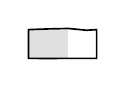
\begin{tikzpicture}
  \node[inner sep=5pt, anchor=west] (b) at (5mm,0)
    {\usebox{\pauseboxsave}};
  \fill[black!12]
    ([xshift=-5mm]b.north west) rectangle (b.south west);
  \draw[decorate, decoration={random steps, segment length=7pt,
    amplitude=0.7pt}, line width=0.6pt]
    ([xshift=-5mm]b.north west) -- (b.north east) --
    (b.south east) -- (b.south west) --
    ([xshift=-5mm]b.south west) -- cycle;
  \end{tikzpicture}\par\medskip}

% compact author block: one names line, one affils line
\makeatletter
\renewcommand\@authorfont{\Large\sffamily}
\renewcommand\@affiliationfont{\normalsize}
\makeatother

\title{Follow Your Strengths: Writing Papers with LLMs}
\subtitle{Paper0, rewritten in ASD-STE100 Simplified Technical
English}
% \note in title breaks headers; working title, timm to confirm.

\author{Tim Menzies\textsuperscript{1},
  Carmen Armenti\textsuperscript{2},
  Dario Di Nucci\textsuperscript{3},\\
  Matteo Esposito\textsuperscript{4},
  Valentina Lenarduzzi\textsuperscript{5},
  Klaus Schmid\textsuperscript{6}}
\affiliation{\institution{%
  \textsuperscript{1}NC State, USA;
  \textsuperscript{2}USI, Switzerland;
  \textsuperscript{3}Univ.~Salerno, Italy;\\
  \textsuperscript{4}Univ.~Oulu, Finland;
  \textsuperscript{5}Univ.~Southern Denmark;
  \textsuperscript{6}Univ.~Hildesheim, Germany\\
  timm@ieee.org; carmen.armenti@usi.ch; d.dinucci@ieee.org;\\
  matteo.esposito@oulu.fi; lenarduzzi@imada.sdu.dk; schmid@sse.uni-hildesheim.de}\country{}}

\begin{abstract}
Paper writing uses time that researchers need for research.
New writers do not have a method that they can follow.
Large language models write quickly, but their text is weak.
This paper gives a method with three parts.
First, machines read the papers of the team and find the strengths of
each member.
Second, the team points those strengths at a topic that the field says
is important.
Third, machines read the literature, and humans review each result at
marked pause points.
This paper is paper0 of this project, rewritten in ASD-STE100
Simplified Technical English~\cite{asdste25}.
\end{abstract}


\keywords{LLM agents, research writing, strengths, experience base,
  science of science}

\begin{document}
\maketitle

\section{Introduction}

\begin{flushright}
{\em If you cannot---in the long run---tell everyone\\ what you have
been doing, your doing has been worthless.}\\ --- Schr\"odinger,
closing a 1950 public lecture~\cite{schrodinger51}
\end{flushright}

Scientists must write papers.\footnote{This paper obeys ASD-STE100
Simplified Technical English~\cite{asdste25}.
Where STE and the usual style rules of this project disagree, STE
wins.
For example, STE lets a sentence start with ``But.''}
Society gives science money, freedom, and trust.
In return, scientists must tell everyone what they found.
Institutions also count papers when they make decisions about money,
jobs, promotion, and graduation.
Thus, for one reason or the other, the writing must occur.

But writing is hard:
\begin{enumerate}
\item New writers need help with the craft of papers.
The known advice is scattered across many years of folklore.
Also, almost none of that advice has tool support.
\item When new writers ask large language models (LLMs) for help, the
models make text that is weak and long.
Many readers call this text ``AI slop.''\footnote{``Slop'' is
machine-made content of low quality, made in large
quantities~\cite{mw25slop}.
One study of 14 million PubMed abstracts found that an LLM touched at
least 10\% of the 2024 abstracts~\cite{kobak24}.
Software developers report the same problem with machine-made code and
documents~\cite{baltes26}.
The term has no agreed definition, but studies now map its
dimensions~\cite{shaib25}.}
\item Older researchers cannot find time for research, because paper
work fills their days.
In software engineering (SE), this load is large.
One SE paper costs more than four times the effort of one machine
learning paper (4.09 against 0.86 ICLR
points~\cite{luo25,menzies26se}).
\end{enumerate}

\begin{figure*}[t]
\centering
\begin{tabular}{c@{\hspace{0.5em}}c@{\hspace{0.8em}}c}
 & {\small\bf AI assistant} & {\small\bf shared document}\\[0.3em]
\raisebox{0.95in}{\small\bf\shortstack{browser only\\(rungs 1--2)}} &
\begin{tikzpicture}[inner sep=0]\node[anchor=south west] (i)
{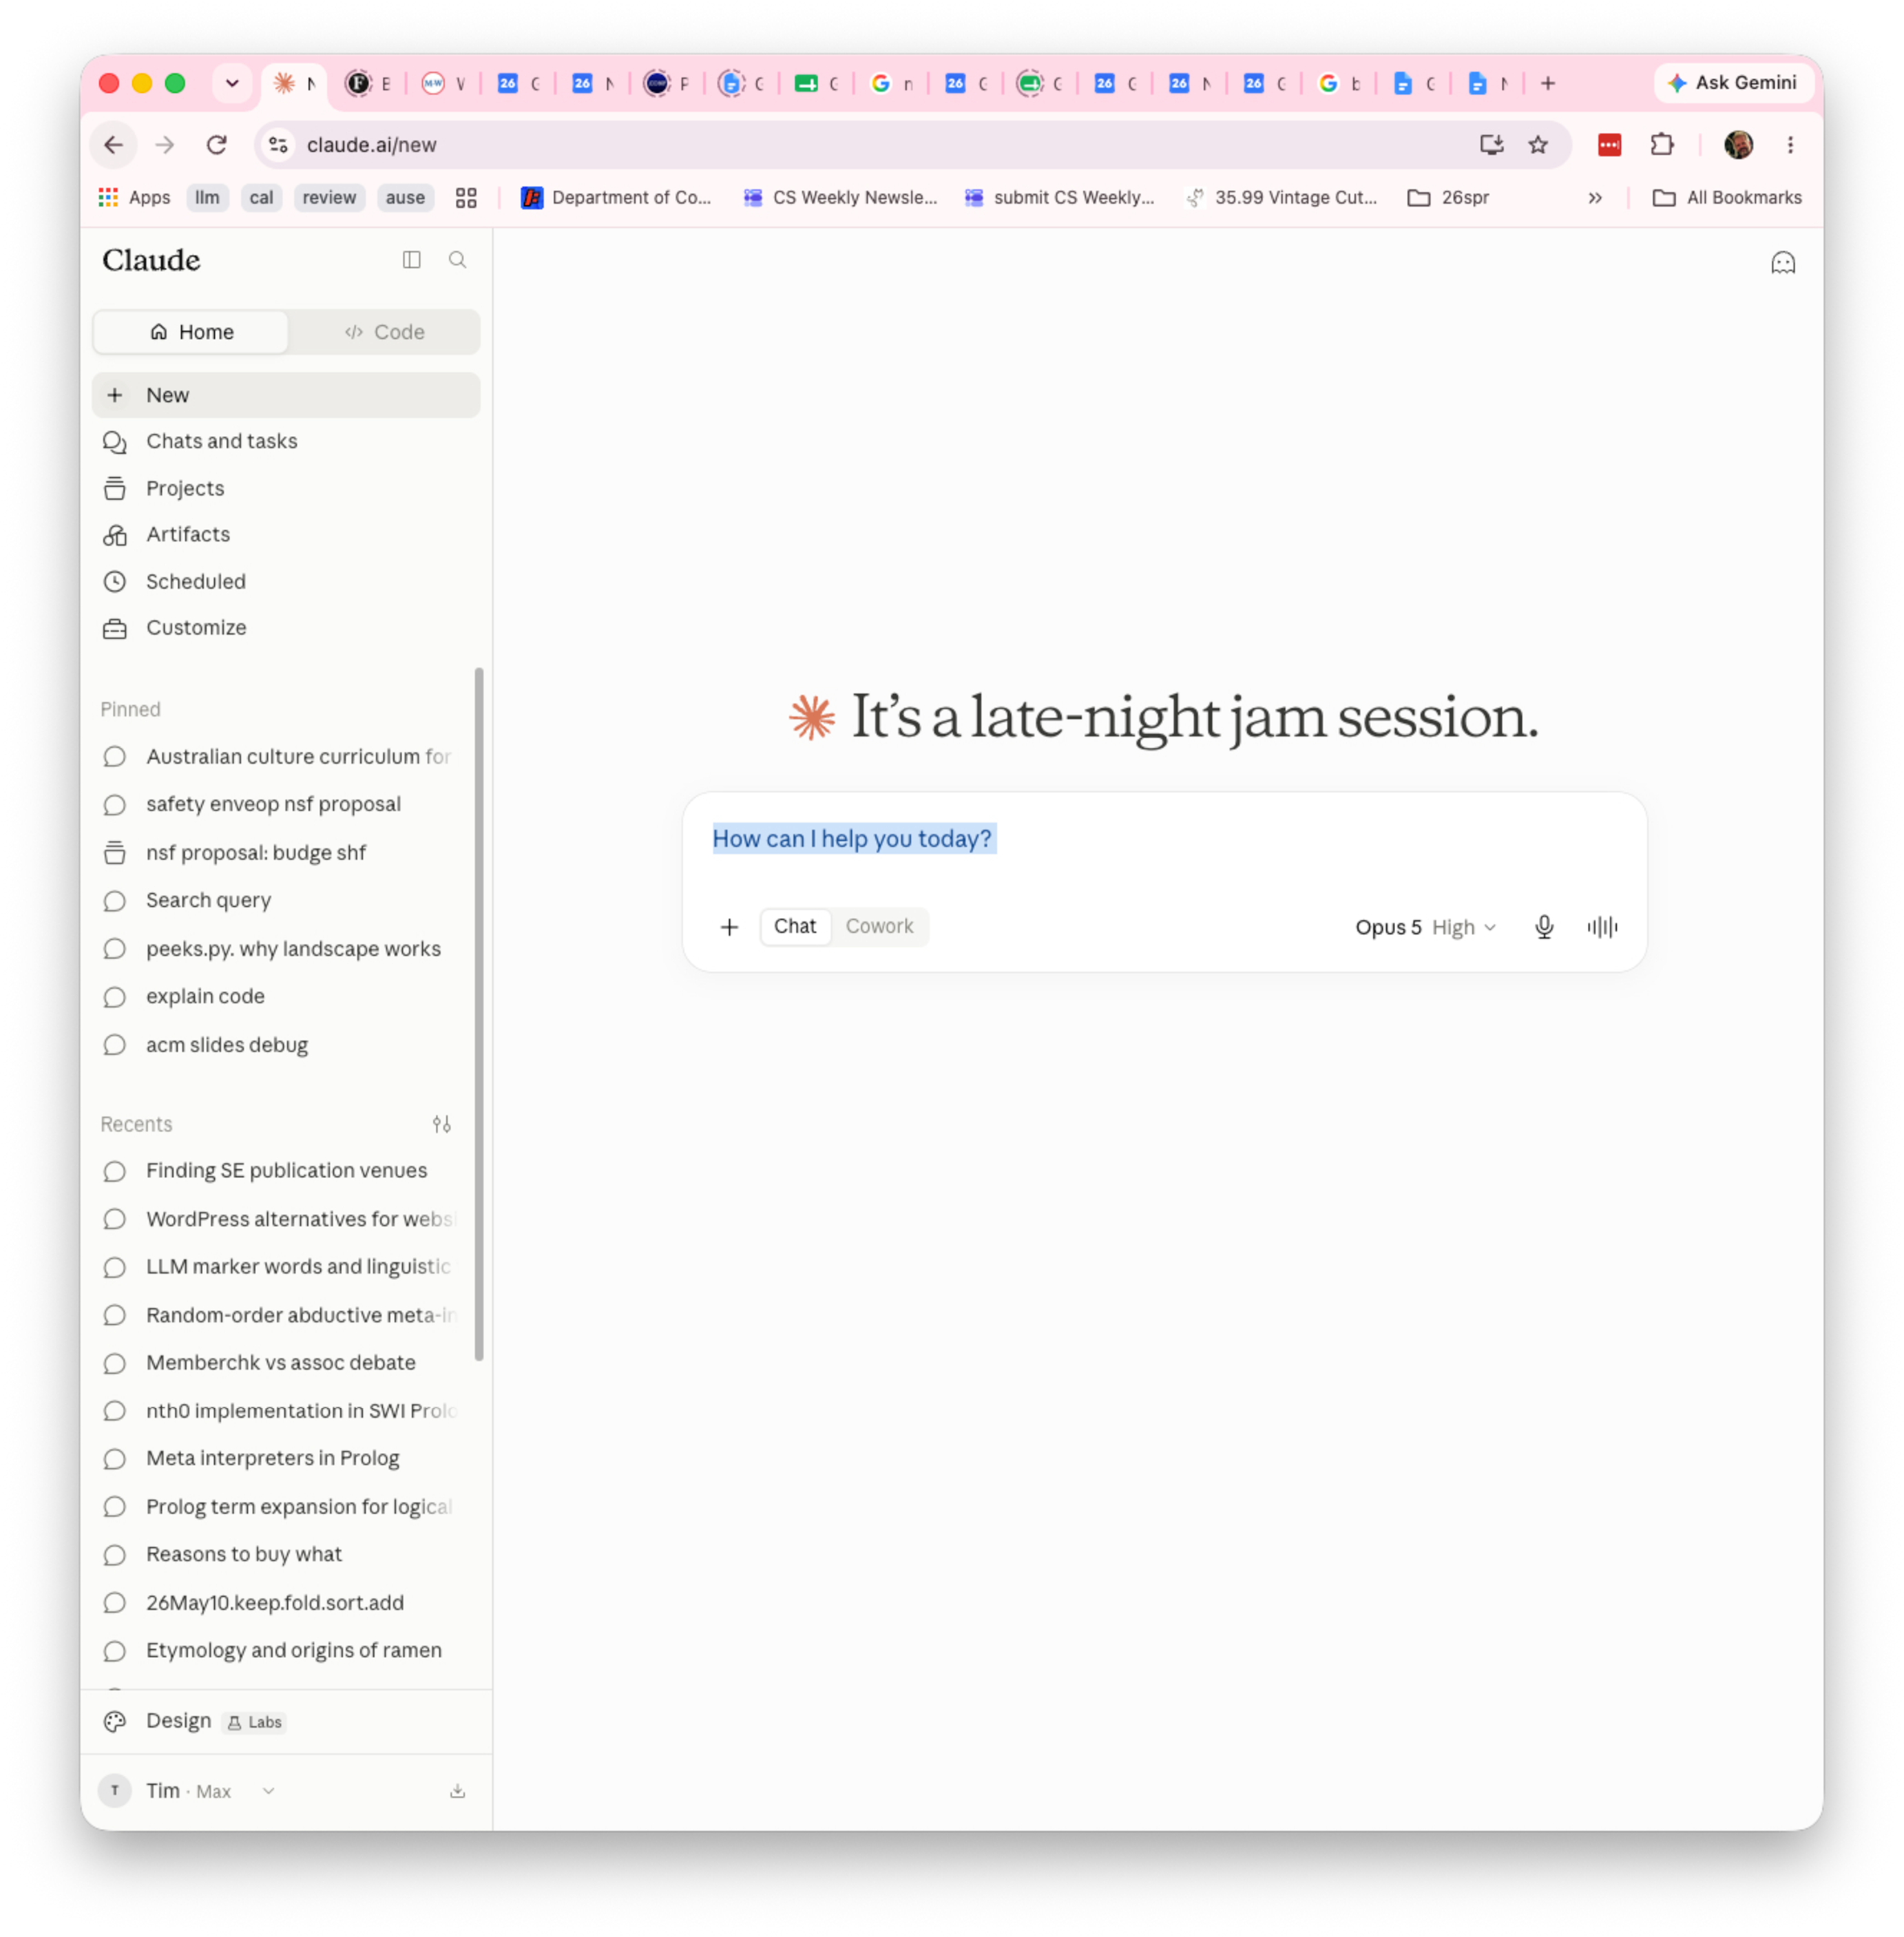
\includegraphics[height=1.9in]{fig/gemini}};\node[anchor=south
west, font=\fontsize{50}{50}\selectfont\bfseries, black] at
([xshift=4mm,yshift=4mm]i.south west) {A};\end{tikzpicture} &
\begin{tikzpicture}[inner sep=0]\node[anchor=south west] (i)
{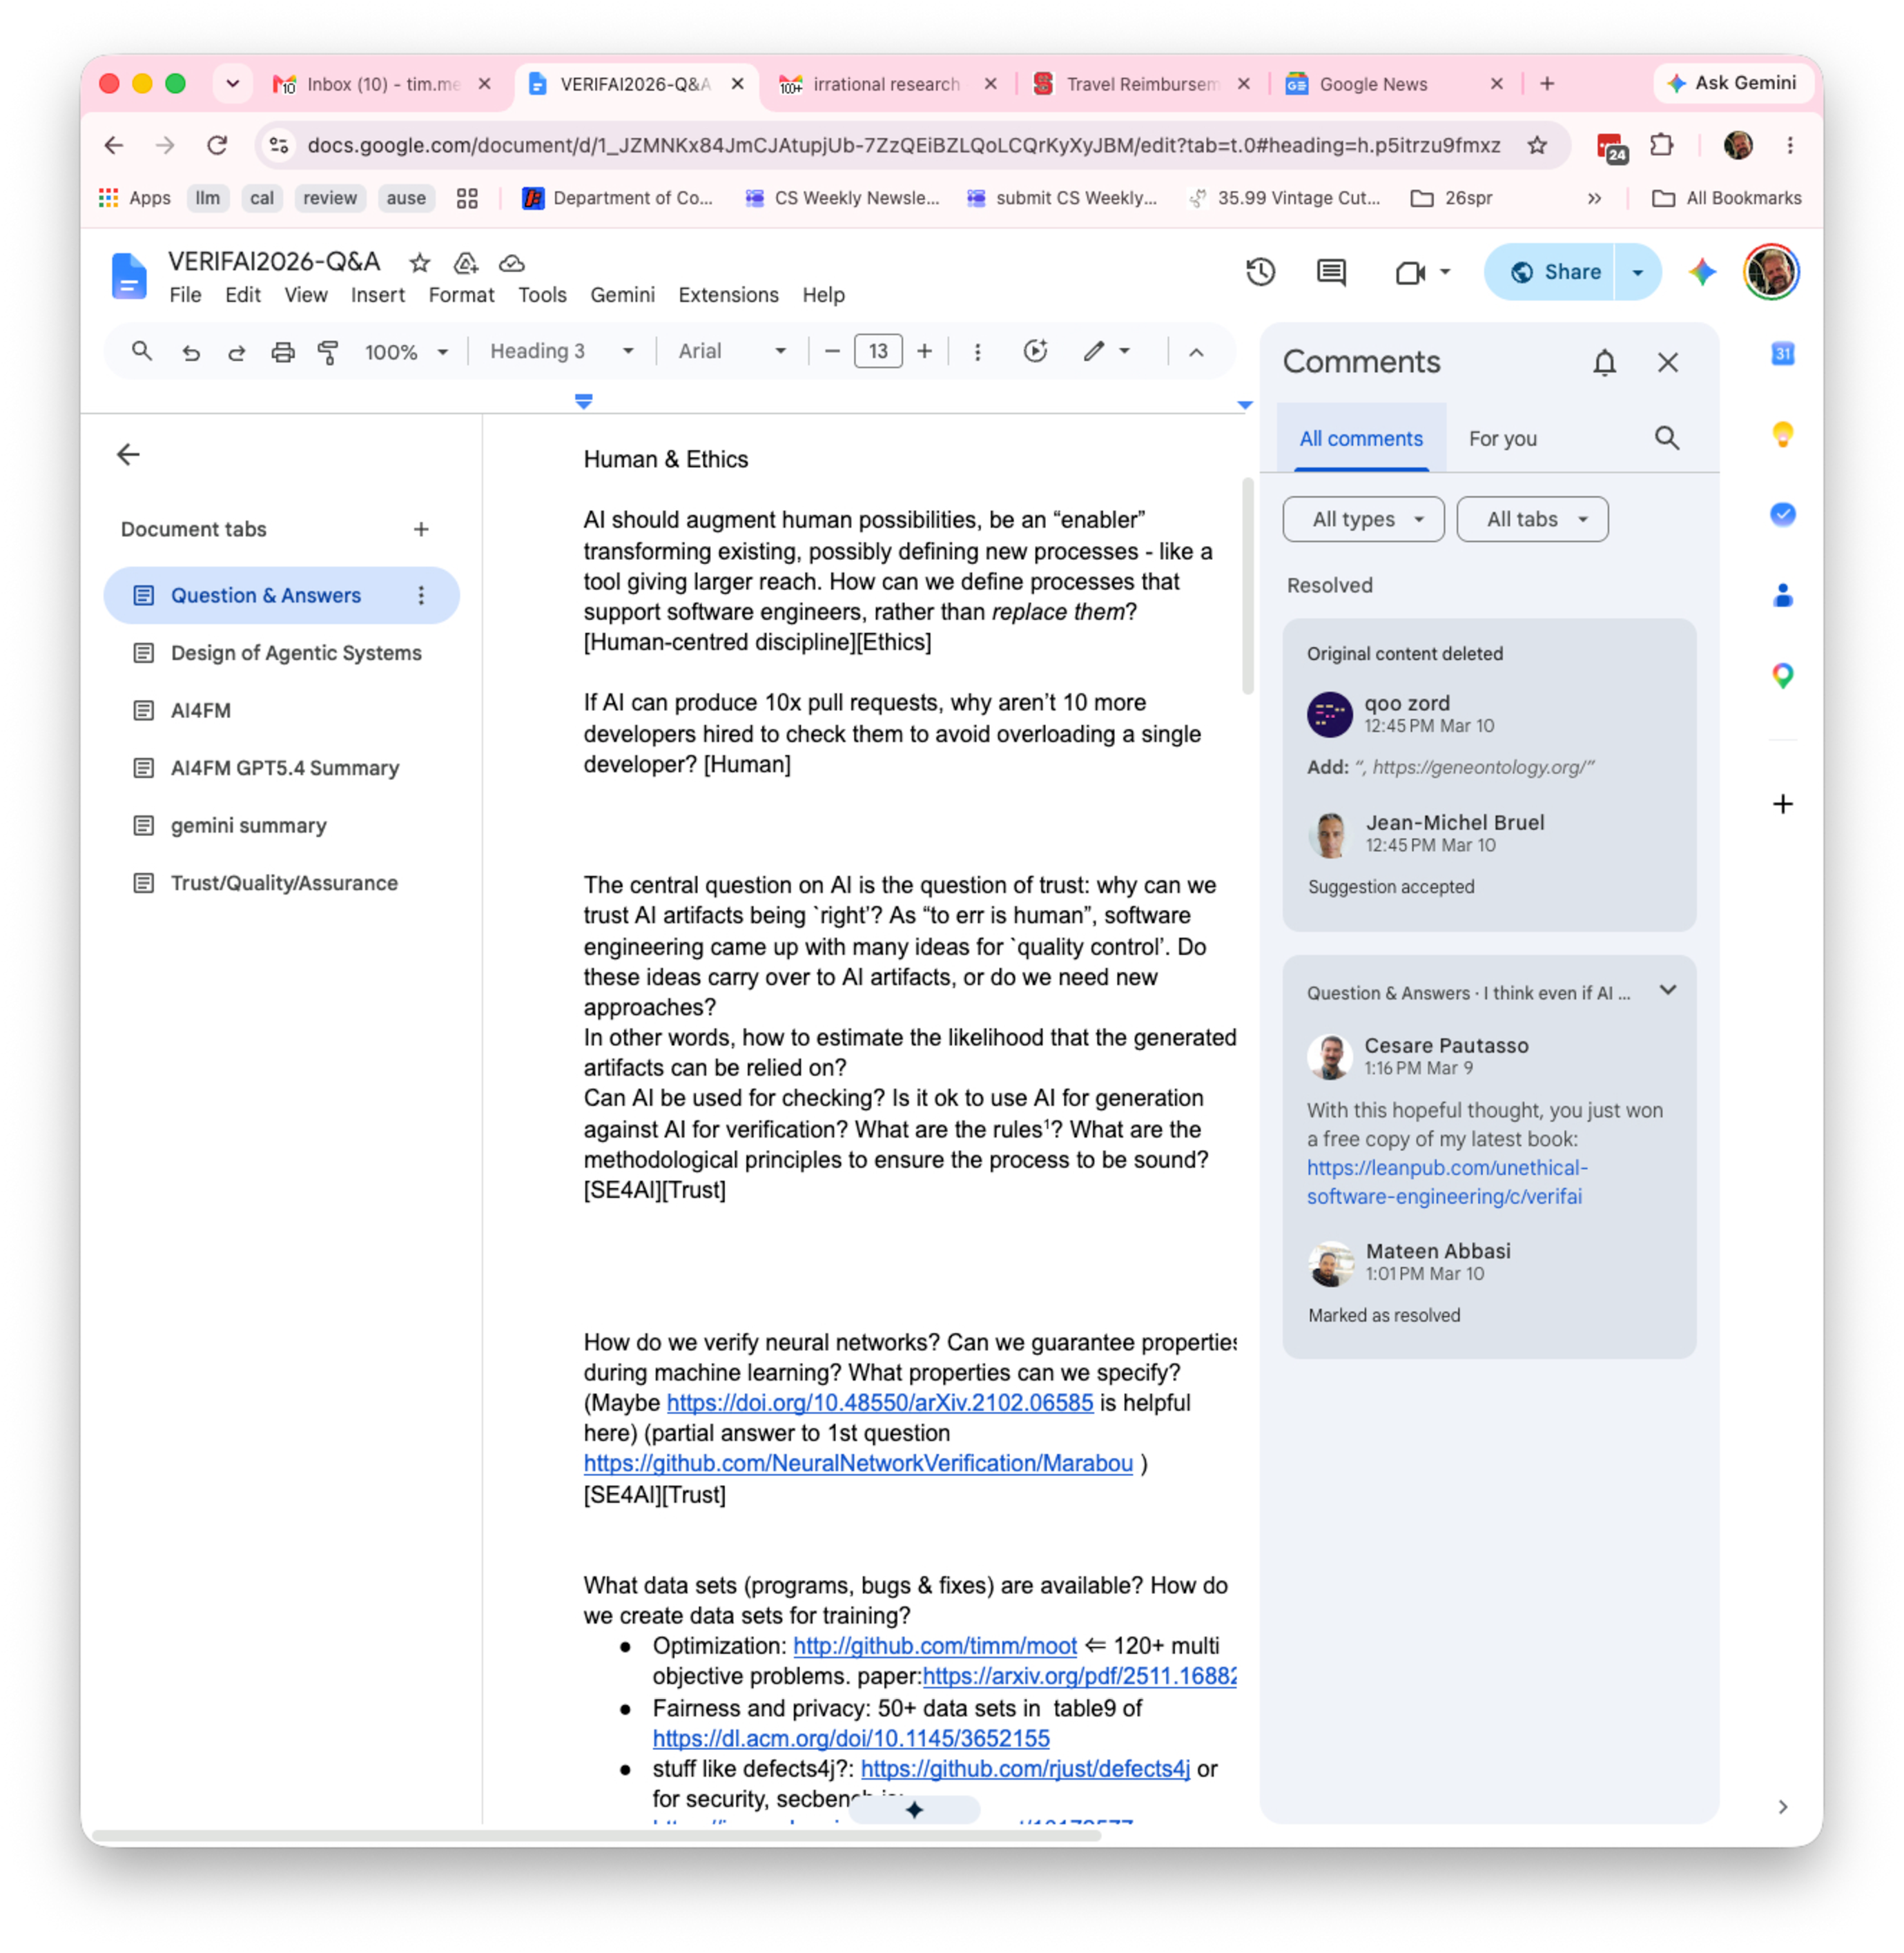
\includegraphics[height=1.9in]{fig/docs}};\node[anchor=south west,
font=\fontsize{50}{50}\selectfont\bfseries, black] at
([xshift=4mm,yshift=4mm]i.south west) {B};\end{tikzpicture}\\[0.6em]
\raisebox{0.95in}{\small\bf\shortstack{repository\\(rungs 3--4)}} &
\begin{tikzpicture}[inner sep=0]\node[anchor=south west] (i)
{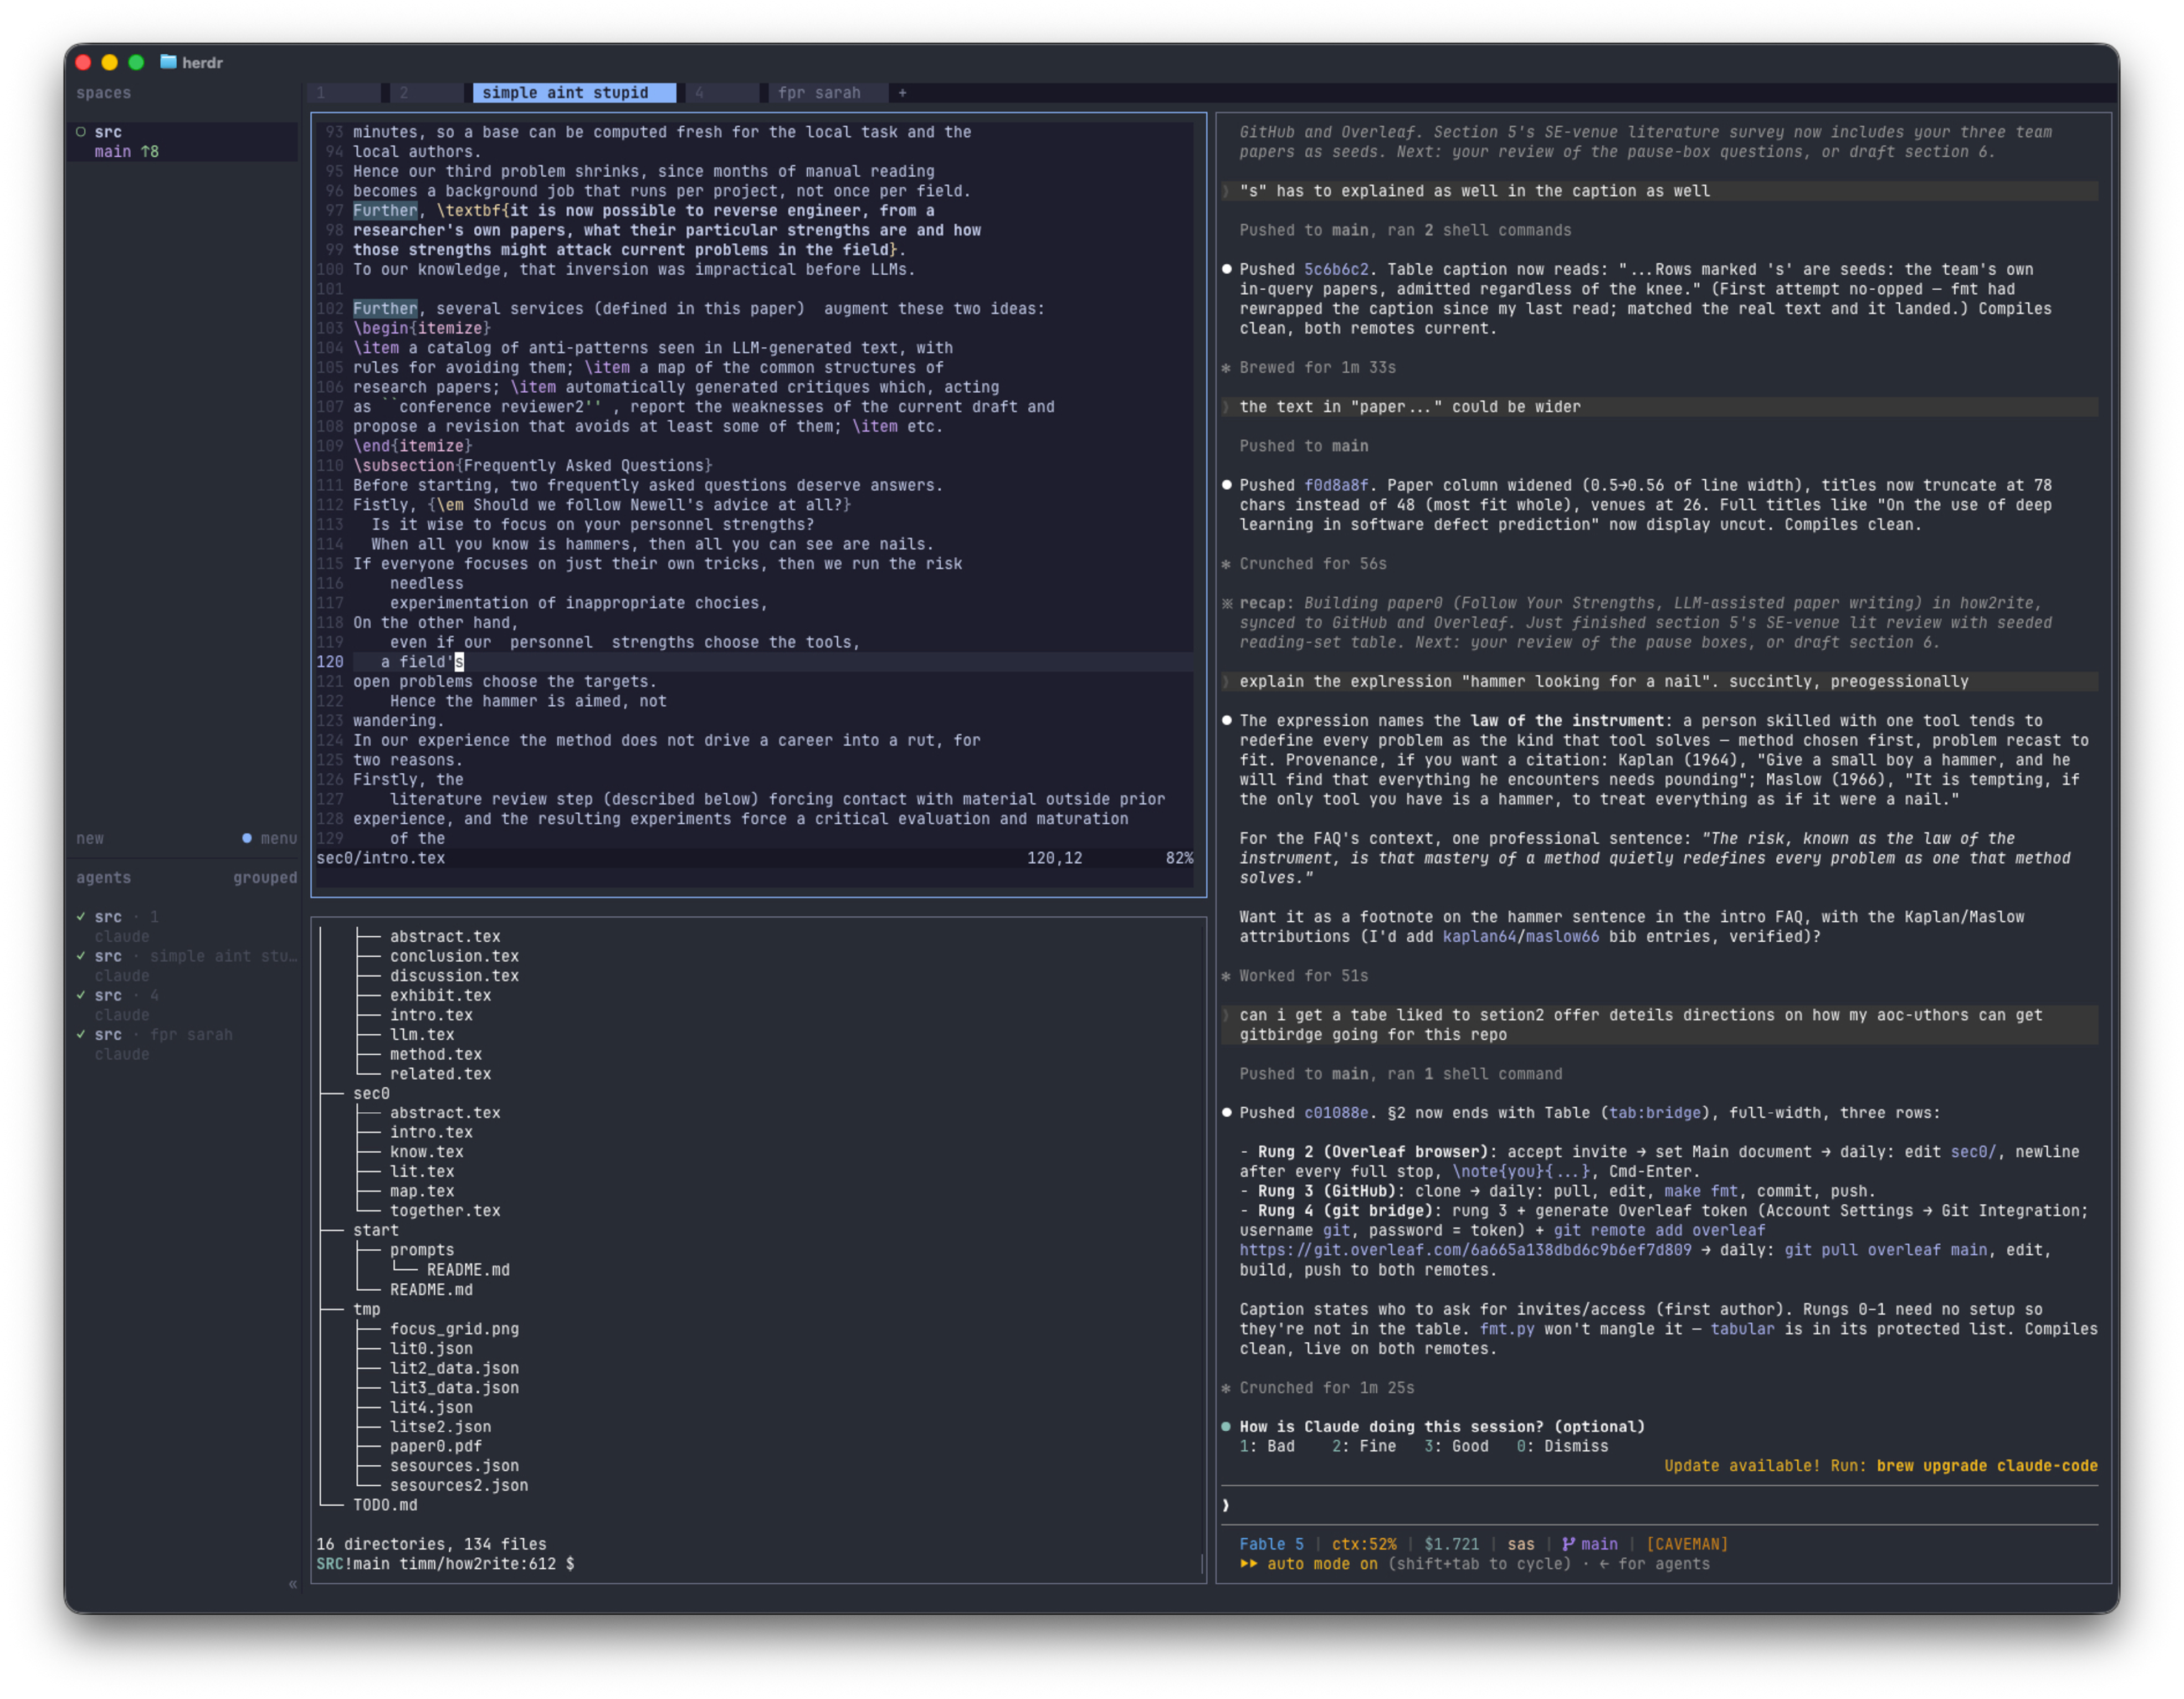
\includegraphics[height=1.9in]{fig/claude}};\node[anchor=south
west, font=\fontsize{50}{50}\selectfont\bfseries, white] at
([xshift=4mm,yshift=4mm]i.south west) {C};\end{tikzpicture} &
\begin{tikzpicture}[inner sep=0]\node[anchor=south west] (i)
{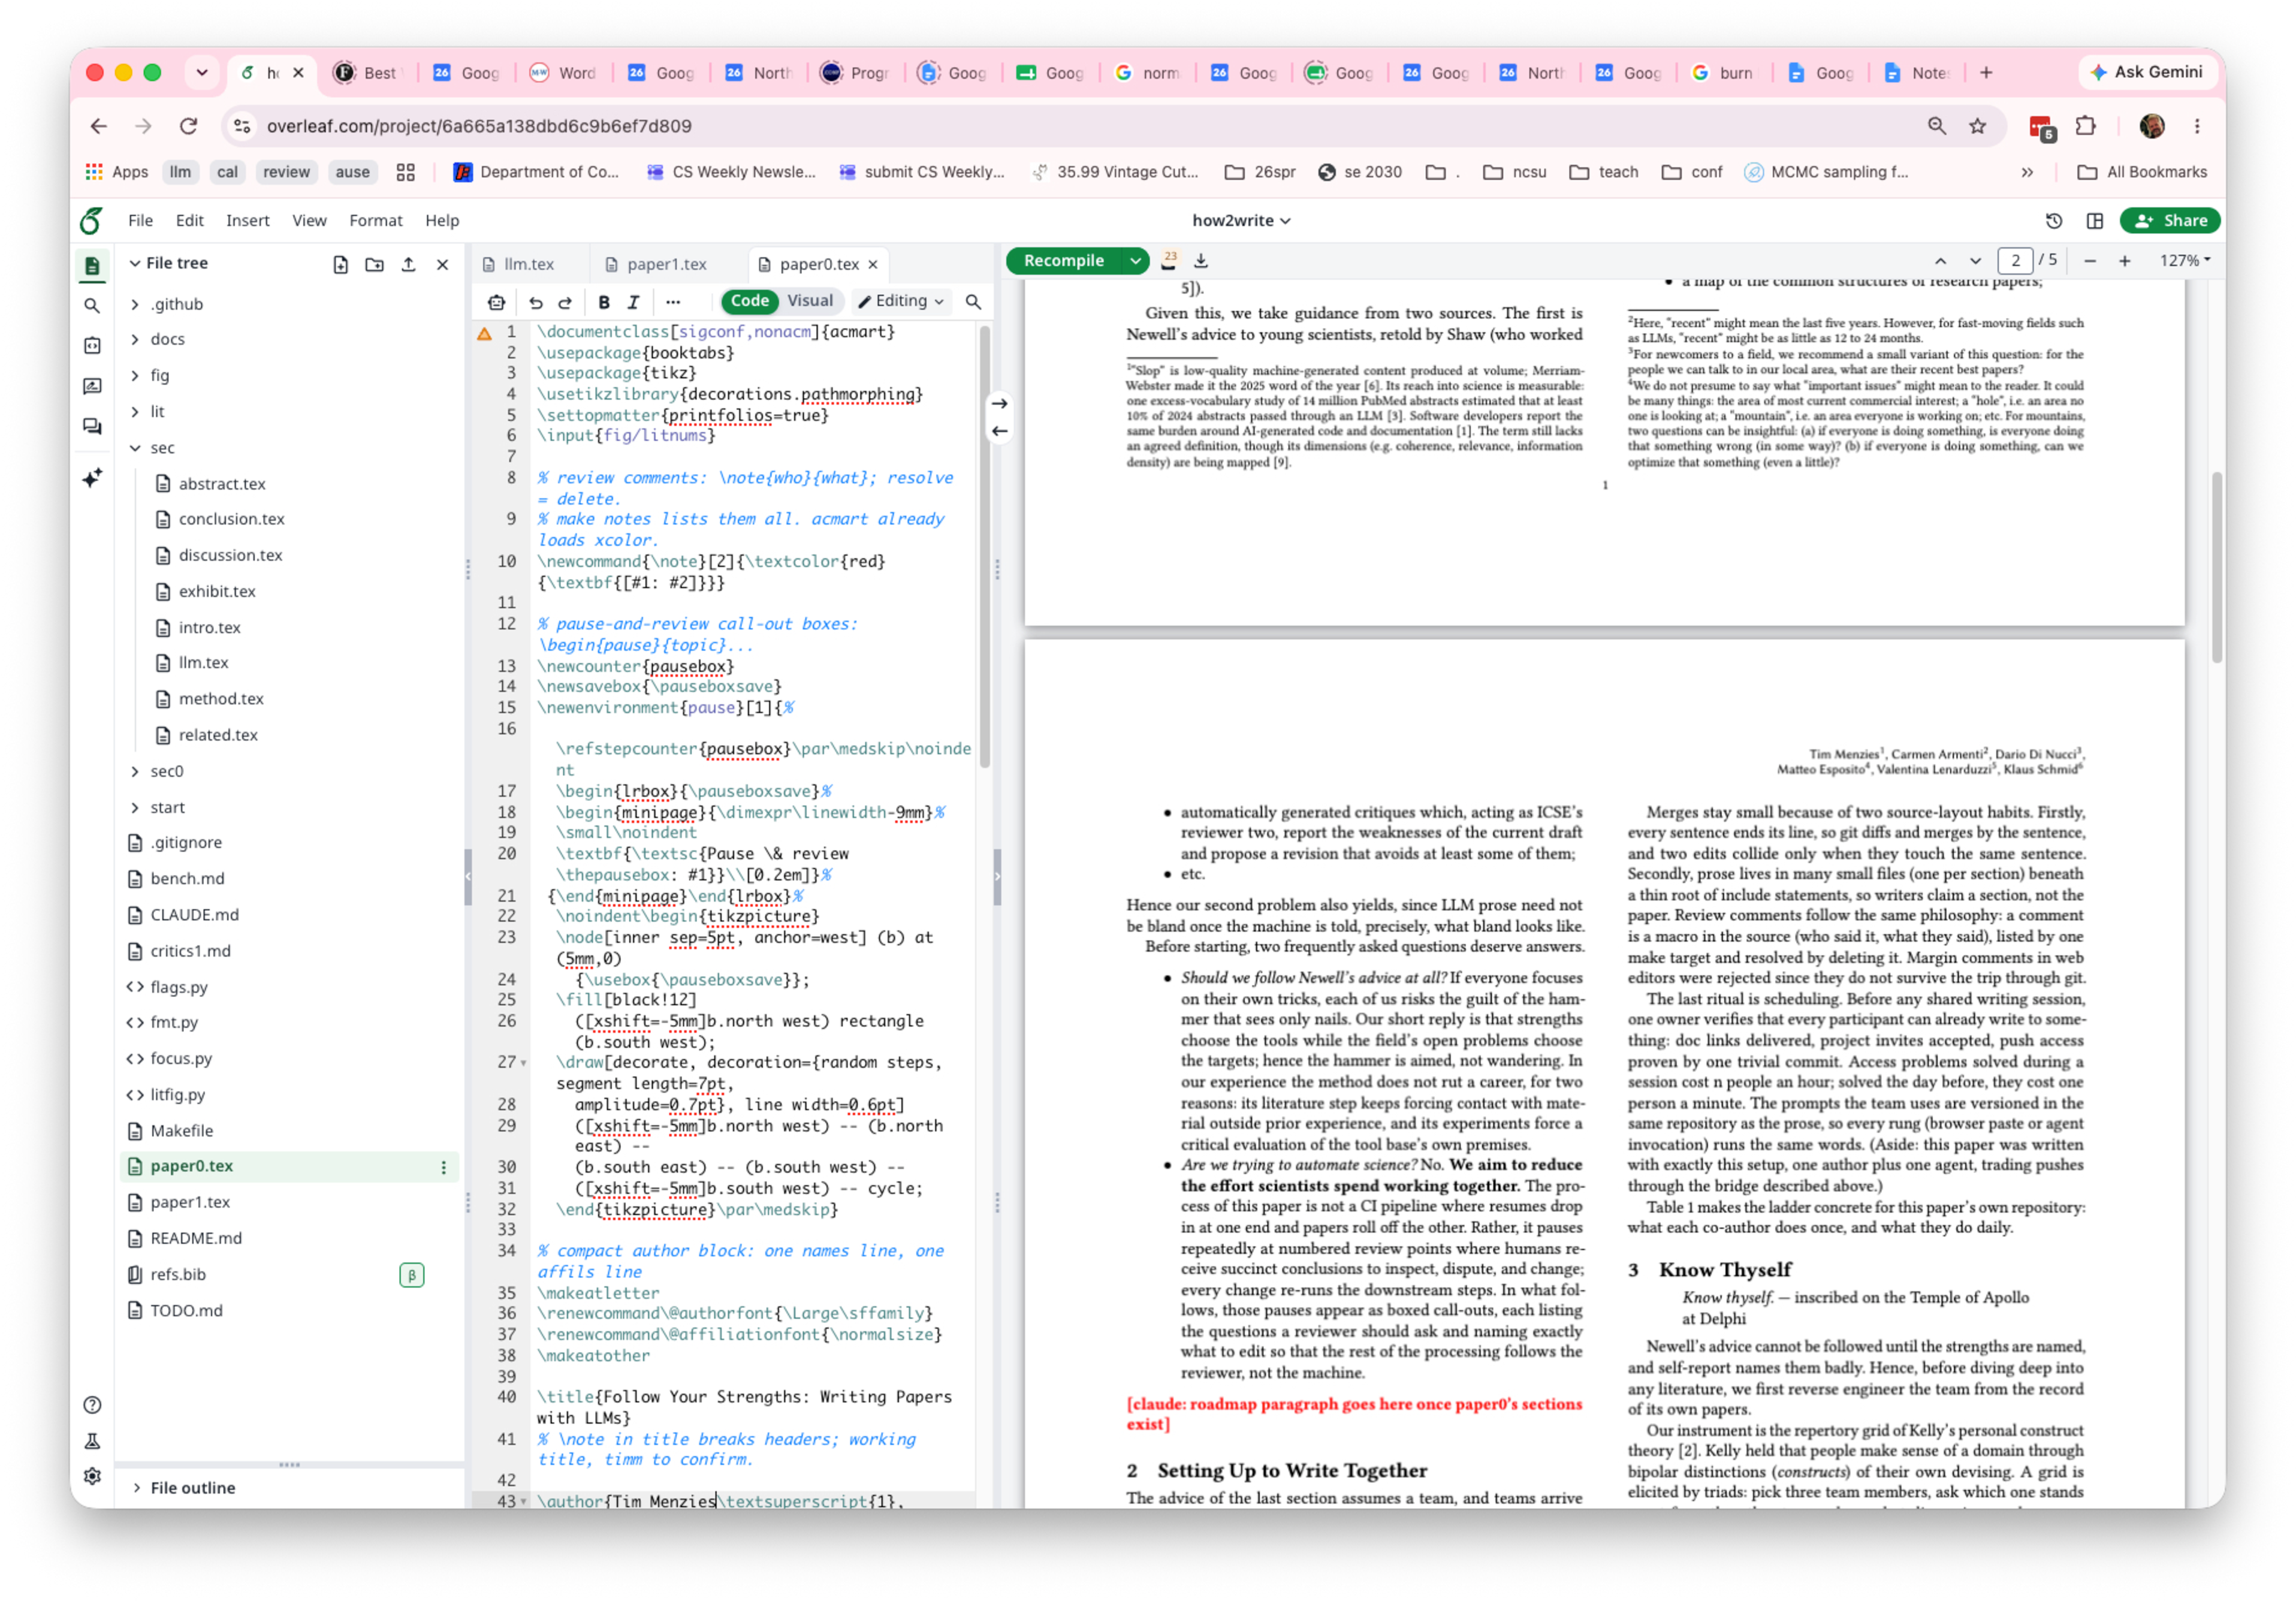
\includegraphics[height=1.9in]{fig/overleaf}};\node[anchor=south
west, font=\fontsize{50}{50}\selectfont\bfseries, black] at
([xshift=4mm,yshift=4mm]i.south west) {D};\end{tikzpicture}\\
\end{tabular}
\caption{Teams can use this advice in many ways.
The columns show AI assistants and shared documents.
The top row shows the browser tools of rungs 1 and 2 (A: Gemini, B:
Google Docs).
The bottom row shows the repository tools of rungs 3 and 4 (C: Claude
Code on the git bridge, D: Overleaf with the same paper).}
\label{fig:faces}
\end{figure*}

Given these problems, we take guidance from two sources.
The first source is the advice of Newell to young scientists.
Shaw worked with Newell at CMU.
She gave this advice again when she answered a question at her FSE'26
keynote~\cite{shaw26}:
\begin{quote}
{\em Know what you are good at.
Work from those strengths, not from your weaknesses.
Then point those strengths at whatever your field currently ranks as
its hardest open problems.} --- after Newell~\cite{newell91}
\end{quote}
Applied to paper writing, this advice gives a workflow of small steps.
It also gives teams a natural division of labor.
Four questions find that division:
\begin{enumerate}
\item ``Hello team: what are our recent best papers?''\footnote{Here,
``recent'' can mean the last five years.
But for fast fields, for example LLMs, ``recent'' can be 12 to 24
months.}
\item ``What do those papers show, through reverse engineering, as our
best strengths?''
\item ``Given those strengths, in which research areas can we work?''
\item ``How can our strengths attack the important issues of those
areas?''\footnote{We do not say what ``important issues'' means for
the reader.
It can be the area with the most commercial interest.
It can be a ``hole,'' an area where no one works.
It can be a ``mountain,'' an area where everyone works.
For mountains, two questions help: (a)~if everyone does one thing, do
they all do it incorrectly in some way?
(b)~if everyone does one thing, can we make that thing better, even a
little?}
\end{enumerate}
Thus, the four questions attack our first problem.
A workflow of clear steps is teachable.
Folklore is not.

The second source is an experience base.
An experience base is a database that machines make from the research
corpus.
It holds, for example:
\begin{itemize}
\item results at the state of the art; \item holes in that state of
the art; \item the test standards of each sub-field; \item other data
of this type.
\end{itemize}
This base is not one size for all.
With LLMs, machines can download and parse hundreds of papers in
minutes.
Thus, a team can compute a fresh base for each task and for each set
of authors.
This attacks our third problem, because months of reading become a
background job for each project.
Also, \textbf{machines can now find, from the papers of one
researcher, the strengths of that researcher}.
Before LLMs, this was not practical.

Several services help these two ideas:
\begin{itemize}
\item a catalog of anti-patterns in LLM text, with rules to avoid
them; \item a map of the usual structures of research papers; \item
automatic critiques that act as ``reviewer 2,'' report the weak points
of a draft, and propose a better draft; \item other services of this
type.
\end{itemize}
Thus, our second problem also becomes smaller.
LLM text does not need to be bland, if we tell the machine what bland
is.

Before we start, we answer two frequent questions.
\begin{itemize}
\item {\em Should we follow the advice of Newell?}
A person who only has a hammer sees only nails, and that is a risk.
But our strengths only select the tools.
The open problems of the field select the targets.
Also, the literature step pushes us to material outside our
experience.
The experiments test the premises of our own tools.
Thus, this method does not lock a career in one place.
\item {\em Do we try to automate science?}
No. \textbf{We try to decrease the effort that scientists spend when
they work together.}
This process is not a pipeline that eats resumes and makes papers.
The process stops at numbered review points.
At each point, a human reads a short conclusion, disputes it, or
changes it.
Each change runs the steps after it again.
\begin{pause}{Pause and reflect}
Boxed call-outs show these pauses.
Each box lists the questions for the reviewer.
Each box names the files to edit, so that the next steps follow the
reviewer, not the machine.
\end{pause}
\end{itemize}

\section{Set Up to Write Together}

The advice of the last section needs a team.
Team members have different comfort with tools.
Some live in the terminal.
Some never used git, and they do not need to.
If we make everyone use one tool, we lose people at both ends.
Thus, we give a ladder, and each author selects a rung:
\begin{enumerate}
\item A reader.
The reader looks at the built PDF and sends comments.
\item A browser writer.
This person writes in a shared Google Doc, with help from claude.ai.
\item An Overleaf writer.
This person edits the LaTeX in the browser and sees the PDF change.
\item A git writer.
This person clones the repository, edits, and pushes.
\item An agent runner.
This person works with an agent, for example Claude Code, on their own
computer.
The agent reads and writes the shared source.
\end{enumerate}
Each rung is a full member of the team.
Only the setup cost is different.

One piece of plumbing connects the ends of the ladder
(Figure~\ref{fig:faces}).
An Overleaf project is also a git remote.
Thus, the same paper has two faces.
Humans see a live editor in the browser.
People and agents see a usual repository.
GitHub holds the source of truth.
A push moves edits to Overleaf in seconds, and a pull collects the
text that the browser writers typed.
Thus, many people and many agents write at the same time, and they
only meet at the merge.

Two habits keep the merges small.
First, each sentence ends its line.
Git then compares texts by the sentence.
Two edits only collide when they touch the same sentence.
Second, the prose lives in many small files, one for each section,
under a thin root of input statements.
Writers then claim a section, not the paper.

Comments follow the same idea.
A comment is a macro in the source.
It shows who spoke and what they said.
One make target lists the open comments.
To resolve a comment, delete it.
We do not use the margin comments of web editors, because those
comments do not go through git.

The last ritual is the schedule.
Before a shared writing session, one owner makes sure that each person
can write to something.
Doc links must arrive.
Project invitations must be accepted.
Push access must be shown with one small commit.
An access problem in a session costs each person an hour.
The same problem, solved one day before, costs one person a minute.

The prompts of the team live in the same repository as the prose.
Thus, each rung runs the same words.
Note: one author and one agent wrote this paper with this method, and
they traded pushes through the bridge above.
Table~\ref{tab:bridge} makes the ladder concrete for this repository.

\begin{table*}[t]
\caption{How to start on this paper, by rung.
The rung 2 writer must get an Overleaf invitation from the first
author.
The rung 3 and 4 writers must get GitHub push access from the same
author.
Each LaTeX rung obeys two habits: start a new line after each full
stop, and keep the prose in many small files under a thin root.}
\label{tab:bridge}
\small
\begin{tabular}{@{}lp{0.42\textwidth}p{0.34\textwidth}@{}}
\toprule
rung & one-time setup & daily cycle\\
\midrule
2: Overleaf browser &
accept the project invitation; open the project; set
{\ttfamily Menu\,$\to$\,Settings\,$\to$\,Main document}
to the paper &
edit the prose in {\ttfamily sec2/}; start a new line after each
full stop; comment with
{\ttfamily \textbackslash note\{you\}\{...\}};
{\ttfamily Cmd-Enter} makes the PDF again\\[0.4em]
3: GitHub &
{\ttfamily git clone github.com/timm/how2rite} &
pull; edit; {\ttfamily make fmt}; commit; push\\[0.4em]
4: the git bridge &
rung 3, plus: in Overleaf, {\ttfamily Account
Settings\,$\to$\,Git Integration\,$\to$\,Generate token} (the
username is {\ttfamily git}, the password is the token); then\newline
{\ttfamily git remote add overleaf}\newline
{\ttfamily ~~https://git.overleaf.com/}\newline
{\ttfamily ~~6a665a138dbd6c9b6ef7d809} &
{\ttfamily git pull overleaf main} (this collects the browser
edits); edit; {\ttfamily make fmt}; build; push to the two remotes:
{\ttfamily git push origin main; git push overleaf main:main}\\
\bottomrule
\end{tabular}
\end{table*}

\begin{pause}{the team's tooling}
Ask: can each team member read and write the files of the paper?
Does each member use a technology where they are productive and
comfortable?
Does the team help everyone, also when system skills are very
different?\\[0.2em] To change the outcome: move people to a different
rung of Table~\ref{tab:bridge} (no rung outranks another), send the
missing invitations or tokens, and name a sync captain who carries
edits between the faces of Figure~\ref{fig:faces}.
\end{pause}

\section{Know Thyself}

\begin{quote}
{\em Know thyself.} --- inscribed on the Temple of Apollo at Delphi
\end{quote}

We cannot follow the advice of Newell before we name the strengths.
Self-report names them badly.
Thus, before we read the literature, we first make machines read us.
The record of our own papers shows the team.

Our instrument is the repertory grid of Kelly~\cite{kelly55}.
Kelly said that people understand a domain through distinctions with
two poles.
He called these distinctions constructs.
Triads make the grid.
Show three team members, then ask which one stands apart, and on which
dimension.
Each answer gives one construct.
Stop when no new dimension appears, then rate each person on each
construct.

Data collection took minutes.
For six authors of this paper, an agent got the five most-cited papers
of all time, and the five most-cited papers of the last five years.
The agent scanned about 1,200 paper records.
It coded the papers against the ICSE'27 research areas.
Then it was the interviewee in the triads.
We merged the constructs that agreed at more than
90\%.\footnote{Caveats: there was one rater (the agent); citation
counts were the only measure of strength; two young authors have few
papers.}
Figure~\ref{fig:focus} shows the result after FOCUS sorting.
Rows and columns move so that similar neighbors touch.
Poles turn so that neighbors align.
Trees join only adjacent clusters.

\begin{figure}[t]
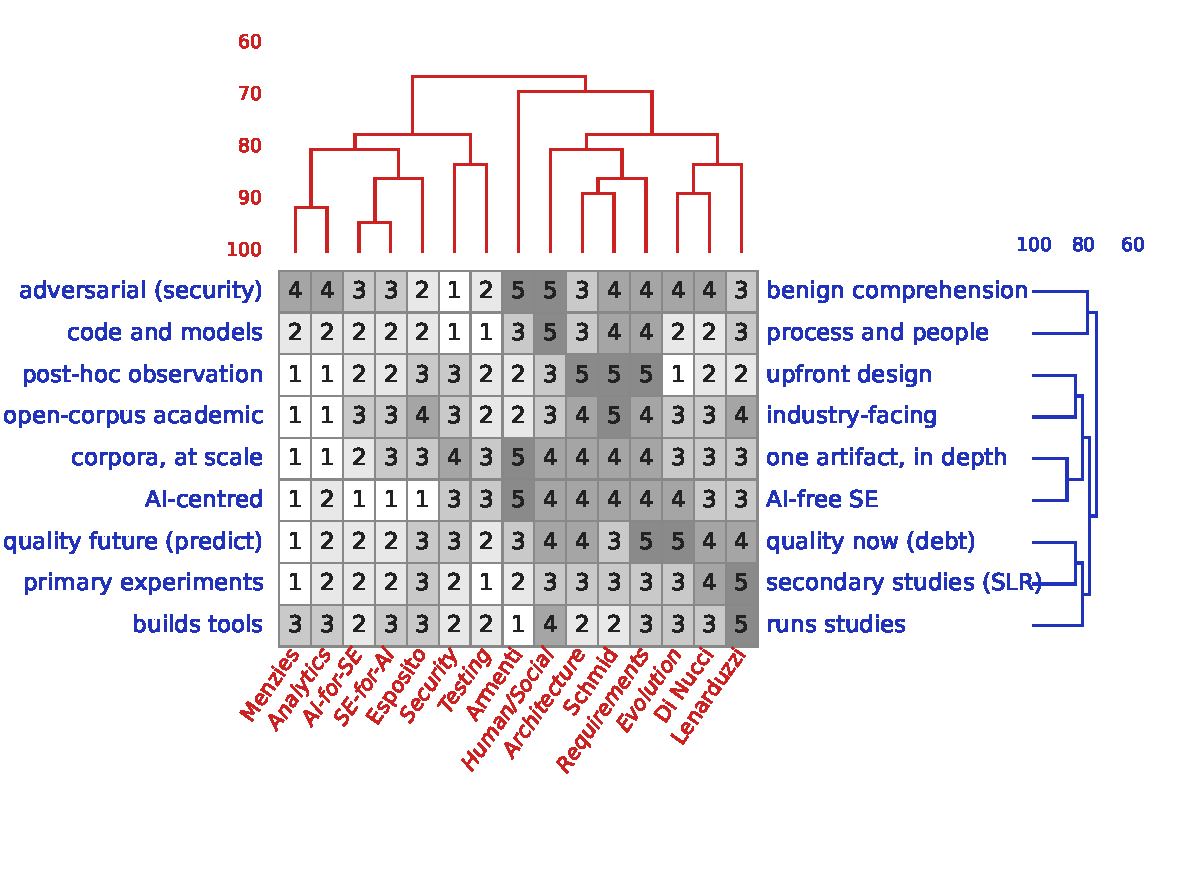
\includegraphics[width=\linewidth]{fig/focus_grid}
\caption{The repertory grid of six authors (upright columns) plus
the nine ICSE'27 areas as reference elements (italic columns; see
\S\ref{sec:map}).
Grey cells score each column from the left pole (1) to the right pole
(5) of each construct.
Trees join neighbors by percentage match.
To make this figure again, use {\em make focus}.}
\label{fig:focus}
\end{figure}

The grid gives three readings.
First, near-synonyms: construct rows that merge early name one
dimension twice.
In this team, corpus-scale work and AI-centred work travel together,
and primary experiments travel with future prediction.
Second, birds of a feather: Lenarduzzi and Di Nucci match at about
90\%.
They are the quality-and-evolution core of the team.
Third, complements: Schmid and Armenti sit far from that core.
Upfront design and single-artifact comprehension are rare skills here,
and one member holds each.

Thus, the grid is two things at one time.
It is a division of labor, and it is a price list of the blind spots
of the team.
We computed it before we read one outside paper.

\begin{pause}{the grid}
Ask: are the construct poles the distinctions that you would make?
Are any ratings unfair to a colleague?
Must we add or remove a person or a construct?
Are five top-cited papers for each author the correct evidence
base?\\[0.2em] To change the outcome: edit the {\ttfamily CONSTRUCTS}
table (or {\ttfamily ELEMENTS}) in {\ttfamily focus.py}, then do
{\ttfamily make focus}; the trees, the pairs of \S\ref{sec:map}, and
the topic arithmetic all follow from that one table.
\end{pause}

\section{Map the Team to the Field}
\label{sec:map}

Questions three and four of Newell ask where a team can work, and
which important issues live there.
For ``where,'' we use the nine areas of the ICSE'27 research track
call for
papers:\footnote{conf.researchr.org/track/icse-2027/icse-2027-research-track}
AI for SE; analytics; architecture and design; dependability and
security; evolution; human and social aspects; requirements and
modeling; SE for AI; and testing and analysis.

We score each area on the same nine constructs as the people.
The areas then join Figure~\ref{fig:focus} as reference elements (the
italic columns).
Each area column is an archetype.
It shows how the usual highly cited researcher of that area scores.
We judged the archetypes from the call for papers, not from a corpus.
\note{claude}{upgrade path: make each area column from its ICSE
distinguished papers of the last five years, coded like the author
papers; then people and areas have one source}

The red tree then answers a question that a topic list cannot answer:
who stands nearest to which area.
Some pairs are strong.
Menzies stands at 92\% match to analytics.
Di Nucci stands at 89\% to evolution.
Schmid stands at 89\% to requirements and to architecture, and
Esposito stands at 86\% to SE for AI.
Some pairs are loose.
The nearest areas of Lenarduzzi (evolution, architecture) reach only
72\%, and the nearest area of Armenti (human and social aspects)
reaches 69\%.
Thus, those two members are less typecast than the rest of us.
Thus, question three answers itself: the natural territory of the team
is the set of areas adjacent to a member.

The far columns are also important.
No author is nearer than 85\% to security (best: Esposito, 78\%) or to
testing (best: 72\%).
Those two areas hold to each other, not to a person.
That is the priced blind spot of this team.
Papers there would go against the grain, or the team needs a new
collaborator who brings that column nearer.

The red tree also shows a larger shape: the team divides in two.
One wing measures.
That wing is Menzies and Esposito, together with analytics and the two
AI areas.
One wing crafts.
That wing is Schmid, Armenti, Di Nucci, and Lenarduzzi, together with
architecture, requirements, human aspects, and evolution.
This split is also a division of labor.
When a paper observes a corpus and builds a thing, each wing takes one
half.

Last, the grid can propose a topic for the full team.
Three calculations use the same matrix: (a)~the area nearest to the
centroid of the six persons (SE for AI and evolution, tied at 83\%);
(b)~the area with the best worst member (evolution, worst member at
64\%); (c)~the midpoint of each pair of areas, scored the same way,
where the best pairs (analytics plus human aspects at 68\%; AI for SE
plus human aspects, average 76\%) beat each single area.
Thus, blends win.
A topic that crosses the two wings serves this team better than one
area.
The best blend is AI for SE crossed with human and social aspects.
That blend describes the paper that you now read.

\begin{pause}{the topic}
Ask: do the archetype columns agree with your reading of the call for
papers?
Would you spend money on the winning blend?
Or must a new collaborator repair the blind spot (security,
testing)?\\[0.2em] To change the outcome: edit the nine area columns
in {\ttfamily focus.py} (or use the area list of a different venue),
then do {\ttfamily make focus}; the centroid, maximin, and blend
scores follow.
\end{pause}

\section{Read In}
\label{sec:lit}

A chosen topic makes a debt: the literature.
Our rules for the literature review are few.
Figure~\ref{fig:prompt} shows the full prompt.
The first three lines are configuration that machines read.
The rules drive the pipeline.

\begin{figure}[t]
\fbox{\parbox{\dimexpr\linewidth-2\fboxsep-2\fboxrule}{\small
{\ttfamily goal:~~human factors of AI assistants\\ \hspace*{4.2em}for
[software engineering]\\ years:~2021-2026\\ seed:~~the team's three
in-query papers}\\[0.4em] Rules: (1)~let the speed of the field set
``recent'': ten years usually, two to three years for LLM-speed
fields; (2)~the term in brackets is a venue filter: the first search
looks only in the venues of that field, from a venue list that a human
can review;\footnote{Sources for the list: se-deadlines.github.io, the
venue index of Google Scholar for ``software engineering,'' OpenAlex
sources with ``software'' in their names, and the venues of the team's
own recent papers.
CORE does not list journals now.}
(3)~sort the hits by citations, and read above the knee of that curve
(the point farthest from the first-to-last chord); (4)~seeds go into
the reading set without a citation test; (5)~the snowball has no venue
filter: it walks backward from the reading set to the classics, and
forward from the seeds to the newest work; (6)~the download rate is a
finding: report it, and never drop missing papers without a word.
Then code each abstract; look for subsets and their overlaps; and list
the papers of the team that already sit inside the set.}}
\caption{The prompt that runs the literature review (from the
search rules of the rite engine, github.com/timm/rite).}
\label{fig:prompt}
\end{figure}

\begin{figure}[t]
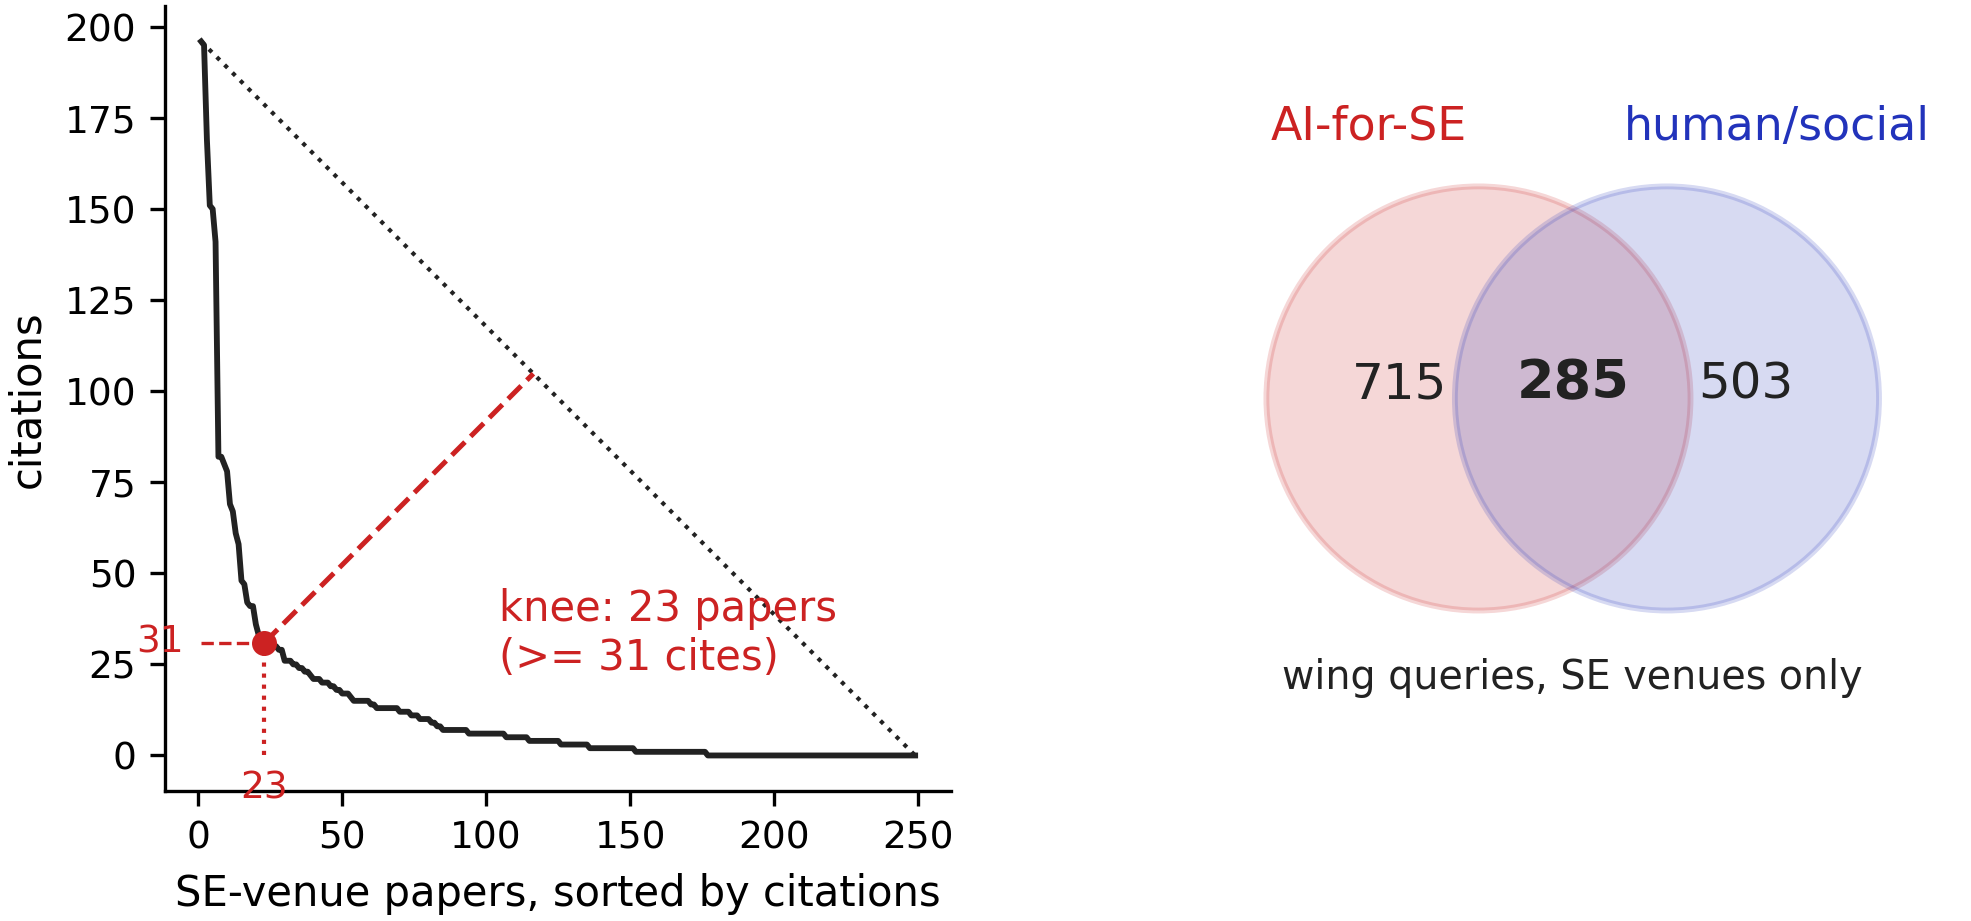
\includegraphics[width=\linewidth]{fig/lit}
\caption{Left: the sorted-cites curve of the goal query, searched
only in SE venues (\litSE{} papers, OpenAlex, 2021--2026).
The dotted line goes from the most-cited to the least-cited paper.
The dashed drop marks the point farthest from that line: the knee,
\litKnee{} papers at \litKneeCites{} citations or more.
Right: the two wings as different queries, with the same venues, and
their \litBoth-paper overlap.
To make this figure again, use {\em make lit}.}
\label{fig:lit}
\end{figure}

Figure~\ref{fig:lit} shows the rules on the area that \S\ref{sec:map}
selected.
The venue rule earned its place two times.
A first draft skipped the rule.
The reading set then filled with general AI blockbusters, and their
venues were far from software engineering.
A second draft filtered the venues after a citation-sorted fetch.
That also failed.
Of the top 1{,}000 hits, only nine sat in SE venues, because papers
with very many citations push out the field before the filter runs.
Thus, the venue list goes into the query itself.
The human hours go only to papers that our field knows.

\begin{figure}[t]
\centering
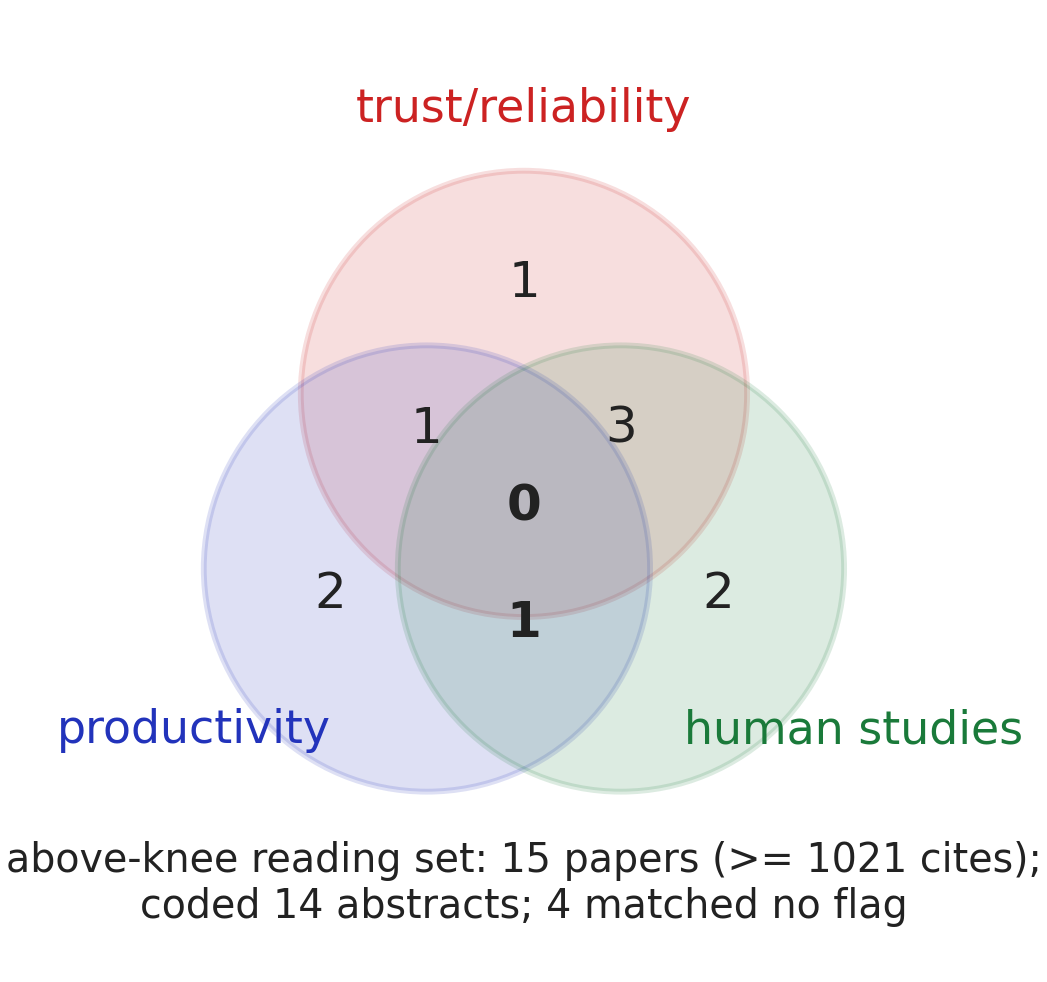
\includegraphics[width=0.62\linewidth]{fig/lit2}
\caption{The reading set (the \litKnee{} papers above the knee of
Figure~\ref{fig:lit}, plus three seeds), coded against three topic
flags.
To make this figure again, use {\em make lit}.}
\label{fig:lit2}
\end{figure}

The reading set is the papers above the knee, plus the seeds.
Rule~(4) admits the seeds without a citation test.
Here, the seeds are the three papers of the team inside the query (the
rows with ``s'' in Table~\ref{tab:read}).
The set has \litRead{} papers, and \litAbs{} of them have abstracts.
Figure~\ref{fig:lit2} codes those abstracts with three topic flags
(trust, productivity, human method).
\litTPH{} papers sit in all three circles, and \litNone{} papers match
no flag.
Table~\ref{tab:read} lists the set and its flags.

\begin{table*}[t]
\caption{The reading set: title (first author), venue, year,
citations, and the three topic flags of Figure~\ref{fig:lit2}.
The rows with ``s'' are seeds: the papers of the team inside the
query, admitted without a citation test. {\em litfig.py} makes this
table from OpenAlex, with the venues as recorded there.}
\label{tab:read}
\scriptsize \setlength{\tabcolsep}{3pt}
\centering
% generated by litfig.py; do not hand-edit
\begin{tabular}{@{}rp{0.58\linewidth}p{0.17\linewidth}rr@{}}
\toprule
\# & paper & venue & year & cites\\
\midrule
1 & Machine Learning: Algorithms, Real-World Application... (Sarker) & SN Computer Science & 2021 & 5221\\
2 & Opinion Paper: “So what if ChatGPT wrote it?” Multid... (Dwivedi) & International Journal  & 2023 & 3869\\
3 & Metaverse beyond the hype: Multidisciplinary perspec... (Dwivedi) & International Journal  & 2022 & 2619\\
4 & Machine learning and deep learning (Janiesch) & Electronic Markets & 2021 & 2534\\
5 & GPT-4 Technical Report (OpenAI) & arXiv (Cornell Univers & 2023 & 2421\\
6 & A Metaverse: Taxonomy, Components, Applications, and... (Park) & IEEE Access & 2022 & 1789\\
7 & Natural language processing: state of the art, curre... (Khurana) & Multimedia Tools and A & 2022 & 1762\\
8 & ARTIFICIAL INTELLIGENCE FOR THE REAL WORLD (?) & International Research & 2023 & 1450\\
9 & A survey on large language model based autonomous ag... (Wang) & Frontiers of Computer  & 2024 & 1284\\
10 & Flamingo: a Visual Language Model for Few-Shot Learn... (Jean-Baptiste) & arXiv (Cornell Univers & 2022 & 1247\\
11 & Generative AI (Feuerriegel) & Business \& Informatio & 2023 & 1241\\
12 & A SWOT analysis of ChatGPT: Implications for educati... (Farrokhnia) & Innovations in Educati & 2023 & 1212\\
13 & A Review of Artificial Intelligence (AI) in Educatio... (Zhai) & Complexity & 2021 & 1168\\
14 & AI-Based Modeling: Techniques, Applications and Rese... (Sarker) & SN Computer Science & 2022 & 1114\\
15 & Hydrogen production, storage, utilisation and enviro... (Osman) & Environmental Chemistr & 2021 & 999\\
16 & Deep learning modelling techniques: current progress... (Ahmed) & Artificial Intelligenc & 2023 & 997\\
17 & The future landscape of large language models in med... (Clusmann) & Communications Medicin & 2023 & 981\\
18 & Unmanned aerial vehicles (UAVs): practical aspects, ... (Mohsan) & Intelligent Service Ro & 2023 & 967\\
19 & A Survey on the Explainability of Supervised Machine... (Burkart) & Journal of Artificial  & 2021 & 966\\
20 & New Era of Artificial Intelligence in Education: Tow... (Kamalov) & Sustainability & 2023 & 956\\
21 & Artificial intelligence and smart vision for buildin... (Baduge) & Automation in Construc & 2022 & 935\\
22 & Using machine learning approaches for multi-omics da... (Reel) & Biotechnology Advances & 2021 & 900\\
23 & A Review of the Role of Artificial Intelligence in H... (Kuwaiti) & Journal of Personalize & 2023 & 838\\
24 & Unlocking the value of artificial intelligence in hu... (Chowdhury) & Human Resource Managem & 2022 & 829\\
25 & A survey on deep learning tools dealing with data sc... (Alzubaidi) & Journal Of Big Data & 2023 & 823\\
26 & Smart wearable devices in cardiovascular care: where... (Bayoumy) & Nature Reviews Cardiol & 2021 & 819\\
27 & Adaptive Learning Using Artificial Intelligence in e... (Gligorea) & Education Sciences & 2023 & 819\\
28 & <scp>ChatGPT</scp> and a new academic reality: <scp>... (Lund) & Journal of the Associa & 2023 & 790\\
29 & Human resource management in the age of generative a... (Budhwar) & Human Resource Managem & 2023 & 790\\
30 & Challenges and Opportunities of Generative AI for Hi... (Michel‐Villarreal) & Education Sciences & 2023 & 780\\
31 & Survey on 6G Frontiers: Trends, Applications, Requir... (Alwis) & IEEE Open Journal of t & 2021 & 776\\
32 & A Review on Large Language Models: Architectures, Ap... (Raiaan) & IEEE Access & 2024 & 738\\
33 & AI Tools in Society: Impacts on Cognitive Offloading... (Gerlich) & Societies & 2025 & 732\\
34 & Academic Integrity considerations of AI Large Langua... (Perkins) & Journal of University  & 2023 & 706\\
35 & ChatGPT and Open-AI Models: A Preliminary Review (Roumeliotis) & Future Internet & 2023 & 697\\
36 & Retrieval-Augmented Generation for Large Language Mo... (Gao) & arXiv (Cornell Univers & 2023 & 686\\
37 & The impact of big data analytics and artificial inte... (Benzidia) & Technological Forecast & 2021 & 675\\
38 & Teachers’ AI digital competencies and twenty-first c... (Ng) & Educational Technology & 2023 & 612\\
\bottomrule
\end{tabular}

\end{table*}

Then the snowball runs from that set.
The snowball has no venue filter, because good ancestors and good
critics live in all venues.
The backward walk found \litRefs{} different references.
Of these, \litClassics{} have two or more citers inside the reading
set, and those are the candidate classics.
The forward walk found \litCiting{} works that already cite the
reading set.
\note{timm}{the three flags are paper0-local; a full run would fork
its own workdir and flags.py, per the engine rules}

The process itself gave findings.
Full texts are rare.
In the companion run of this workdir, only 22 of 54 wanted PDFs (41\%)
downloaded.
Abstracts come more easily (here, \litAbs{} of \litRead).
Google Scholar does not speak to scripts.
OpenAlex, Semantic Scholar, and arXiv answer machine queries.
Thus, the pipeline stands only on the willing.
An earlier full-text pass showed that abstract-only coding missed
about half of the flags.
Thus, we code the full text above the knee.
Last, the own-papers rule paid.
Three papers of this team already sit in the results (Di Nucci on
accessibility, Schmid on MLOps, Esposito on AI agents).
The territory is adjacent to us, but we do not occupy it yet.

\begin{pause}{the search}
Ask: are the goal line and the two wing queries the correct words?
Is 2021 the correct floor for ``recent''?
Is the venue list (see the box) the SE that you know?
Are the three coding flags your vocabulary, and is a knee that keeps
\litKnee{} of \litSE{} papers too greedy?\\[0.2em] To change the
outcome: edit the query strings, {\ttfamily VENUES}, and {\ttfamily
FLAGS} in {\ttfamily litfig.py}; remove the cache in {\ttfamily tmp/};
then run again.
The two figures, the table, and each number in this section change
with them.
\end{pause}


\bibliographystyle{ACM-Reference-Format}
\bibliography{refs}

\end{document}
